
We now complement our asymptotic analysis with a simulation study designed to evaluate the behavior of $\alpha$RTS designs. The implementation and simulation scripts used in this study can be accessed at \url{https://github.com/ryagouti/rebalancing-targeting-strategies}.

	Our experiments address three questions. First, we investigate the
	convergence of allocation proportions and plug-in target estimates in a
	three-treatment setting (\(K=3\)). Second, we study the impact of forced
	exploration when the target allocation is sparse. Finally, we evaluate the
	performance of hypothesis testing procedures based on data collected with
	\(\alpha\)RTS and \(\alpha\)RTS-FE designs in a four-treatment setting
	(\(K=4\)). Together, these experiments illustrate both the allocation
	properties and the inferential performance of the proposed methods.
	
	We set \(\alpha=0.4\) throughout the experiments. This choice follows the recommendation of \cite{hu2009efficient}, who suggest values of \(\alpha\) between \(0.4\) and \(0.7\)
	based on their numerical study of ERADE.

\subsection{Convergence of Allocation Proportions and Plugin Estimate}

The first experiment is designed to illustrate the convergence behavior predicted by Theorems \ref{thm:LLN} and \ref{thm:normality-gen-erade}. We consider a three-treatment setting (\(K=3\)) with Bernoulli arms with success probabilities $\Theta=(0.5, 0.6, 0.8)$, and use the Neyman allocation as the target, defined as
\[\rho_k^N(\Theta) = \frac{\sqrt{\theta_k(1-\theta_k)}}{\sum_{\ell=1}^{K}\sqrt{\theta_{\ell}(1-\theta_{\ell})}}\;.\]
For two-arms the Neyman allocation (\cite{neyman1934representative}) is the one minimizing the variance of the estimator of the treatment difference as shown in \cite{melfi1998variablility}, and its natural extension to $K$ arms can be traced back to \cite{Cochran1977}.

Figures \ref{fig:fixed-tgt-prop} and \ref{fig:fixed-tgt-plugin} respectively  display  the evolution of the absolute errors $|N_{n,k}/n - v_k|$ and $|\hat{\rho}_{n,k} - v_k|$ as a function of $n$, for the three example of $\alpha$RTS design discussed in Section~\ref{sec:alpha-rts}: Distance-Based, ERADE 2025 and Interpolated D-Tracking. Across all treatments, both quantities decrease rapidly as the sample size increases, indicating that the allocation proportions track the target allocation and that the plug-in estimator stabilizes. This behavior is consistent with the almost sure convergence results  implied by Theorems \ref{thm:LLN} and \ref{thm:normality-gen-erade}. While all three designs share the same asymptotic guarantees, we observe minor differences in early-stage variability. The D-Tracking rule exhibits larger fluctuations at small sample sizes, due to its more aggressive reallocation strategy, whereas the distance-based and ERADE-type rules yield smoother trajectories. These differences vanish as $n$ increases, and all methods display similar behavior in later stages.

\begin{figure}[tb]
	\centering
	\begin{subfigure}[t]{0.32\linewidth}
		\centering
		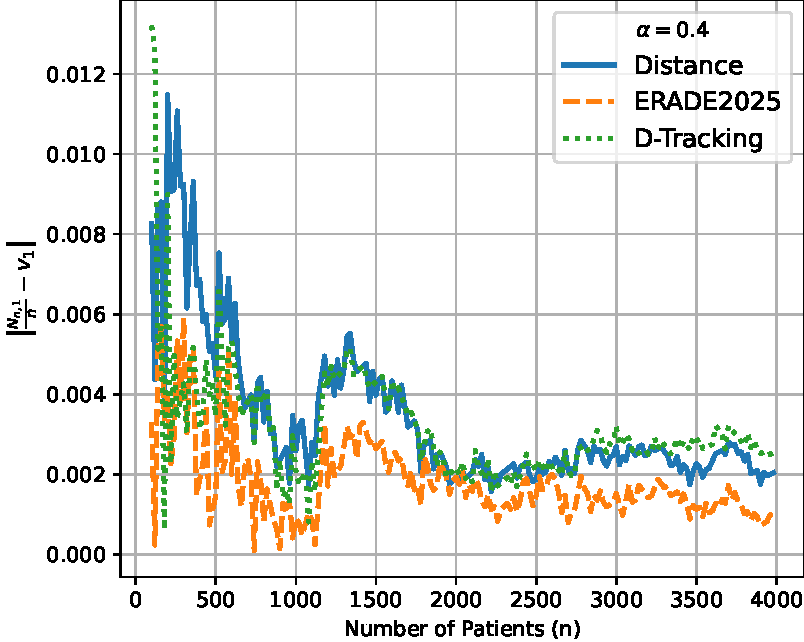
\includegraphics[width=\linewidth]{plots/fixed_target/prop_diff_0.pdf}
		\caption{Treatment 1}
	\end{subfigure}
	\hfill
	\begin{subfigure}[t]{0.32\linewidth}
		\centering
		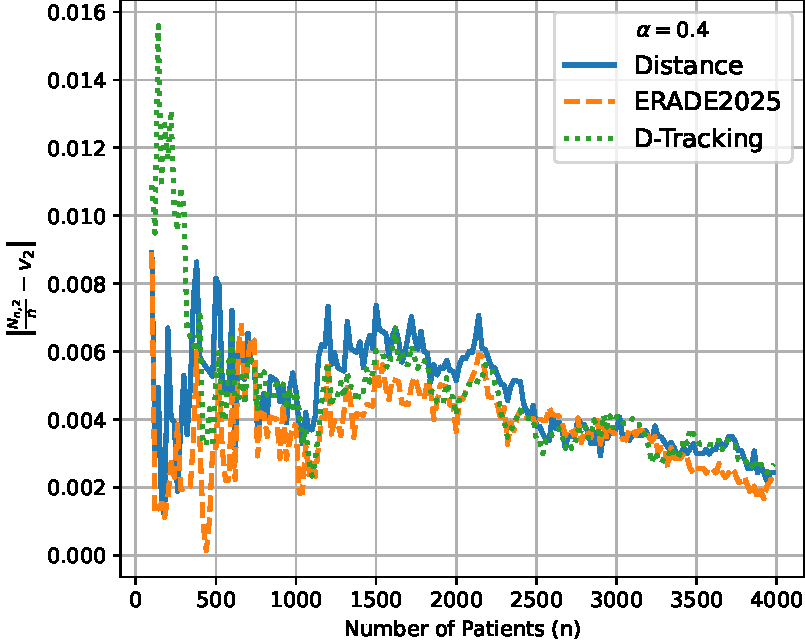
\includegraphics[width=\linewidth]{plots/fixed_target/prop_diff_1.pdf}
		\caption{Treatment 2}
	\end{subfigure}
	\hfill
	\begin{subfigure}[t]{0.32\linewidth}
		\centering
		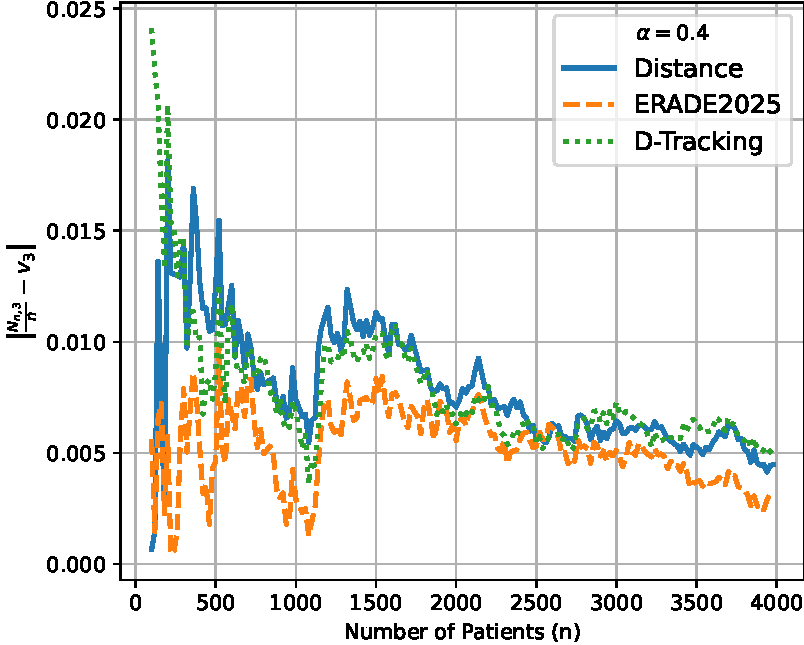
\includegraphics[width=\linewidth]{plots/fixed_target/prop_diff_2.pdf}
		\caption{Treatment 3}
	\end{subfigure}
	
	\caption{Distance between the empirical allocation proportion and the target as a function of $n$ for different $\alpha$RTS designs targeting the Neyman Allocation}
	\label{fig:fixed-tgt-prop}
\end{figure}



\begin{figure}[tb]
	\centering
	\begin{subfigure}[t]{0.32\linewidth}
		\centering
		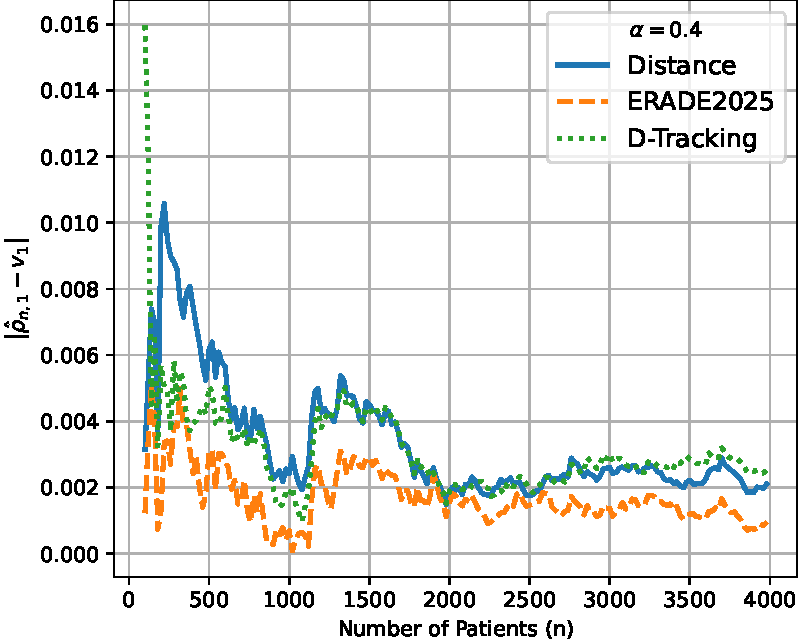
\includegraphics[width=\linewidth]{plots/fixed_target/rho_diff_0.pdf}
		\caption{Treatment 1}
	\end{subfigure}
	\hfill
	\begin{subfigure}[t]{0.32\linewidth}
		\centering
		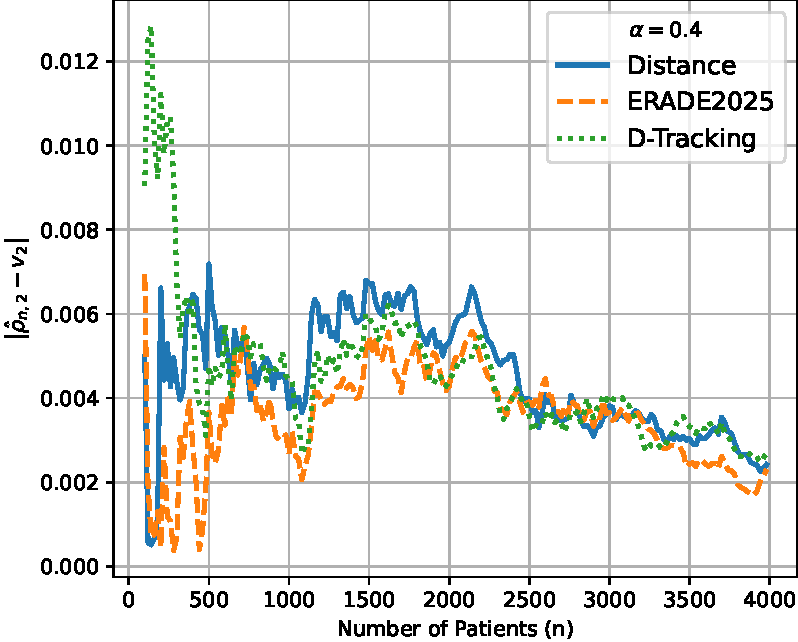
\includegraphics[width=\linewidth]{plots/fixed_target/rho_diff_1.pdf}
		\caption{Treatment 2}
	\end{subfigure}
	\hfill
	\begin{subfigure}[t]{0.32\linewidth}
		\centering
		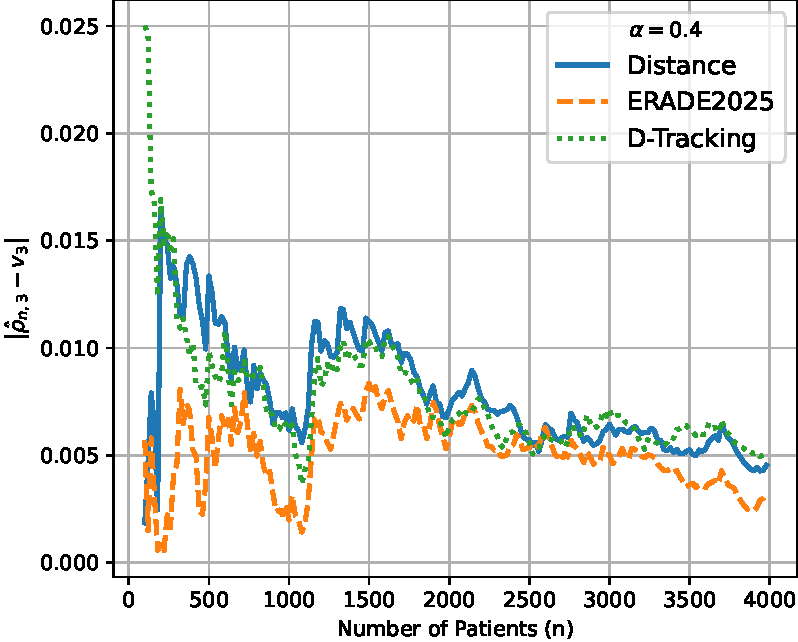
\includegraphics[width=\linewidth]{plots/fixed_target/rho_diff_2.pdf}
		\caption{Treatment 3}
	\end{subfigure}
	
	\caption{Distance between the target plug-in estimate and the target as a function of $n$ for different $\alpha$RTS designs targeting the Neyman Allocation}
	\label{fig:fixed-tgt-plugin}
\end{figure}

\subsection{The Impact of Forced Exploration} Our second experiments aims at illustrating the impact of forced exploration when the target allocation is sparse.
The work of \cite{tymofyeyev2007implementing} proposes a family of target allocations in multi-treatment Bernoulli experiments that are motivated by homogeneity tests, that is, testing
the equality of treatment success probabilities across all arms. In this work, we consider the allocation that minimizes the sample size given a constraint on the power of the homogeneity test (which can be related to a constraint on the non-centrality parameter of some chi-square distribution). This target allocation is shown to exhibit a sparsity pattern for a wide range of parameter configurations. In particular, if $\Theta$ is such that
\[\theta_1=\cdots=\theta_s
>
\theta_{s+1}\geq\cdots\geq \theta_{K-g}
>
\theta_{K-g+1}=\cdots=\theta_K ,\]
then
\[
\rho_i^T(\Theta)=
\begin{cases}
	\displaystyle
	\frac{\sqrt{\theta_1 (1 - \theta_1)}}
	{s\left(\sqrt{\theta_1 (1 - \theta_1)}+\sqrt{\theta_K (1 - \theta_K)}\right)},
	& \text{if } i\in\{1,\dots,s\},
	\\[1.2em]
	0,
	& \text{if } i\in\{s+1,\dots,K-g\},
	\\[1.2em]
	\displaystyle
	\frac{1}{g}\left(
	1-
	\frac{\sqrt{p_1q_1}}
	{\sqrt{p_1q_1}+\sqrt{p_Kq_K}}
	\right),
	& \text{if } i\in\{K-g+1,\dots,K\}.
\end{cases}
\]
and \(\rho_{s+1}^T=\cdots=\rho_{K-g}^T=0\). This allocation, which we call the Tymofyeyev allocation in our study, assigns positive target proportions only to the best-performing and the worst-performing treatments. 

%We remark that it coincides with an allocation minimizing the variance of the difference between these two extreme treatments.

In our experiments, we consider a trial with $K=3$ arms and binary responses. The success probabilities are chosen from the following configurations
\[\Theta=(\theta_1,\theta_2,\theta_3) \in \{(0.1,0.3,0.6), (0.3,0.4,0.7), (0.4,0.6,0.8)\}\]
which induce sparse Tymofyeyev target allocations with treatment 2 being intermediate and asymptotically eliminated. The target values \(\rho^{T}\left(\Theta\right)\) for these instances are reported  in Table~\ref{tab:rho_tymo}.

\begin{table}[b]
	\centering
	\begin{tabular}{c|ccc}
		\hline
		$(\theta_1,\theta_2,\theta_3)$ & Arm 1 & Arm 2 & Arm 3 \\
		\hline
		$(0.1,\,0.3,\,0.6)$ & 0.3798 & 0 & 0.6202 \\
		$(0.3,\,0.4,\,0.7)$ & 0.5000 & 0 & 0.5000 \\
		$(0.4,\,0.6,\,0.8)$ & 0.5505 & 0 & 0.4495 \\
		\hline
	\end{tabular}
	\caption{\label{tab:rho_tymo}Tymofyeyev target allocation vectors corresponding to different instances $\Theta$}
\end{table}

We compare \(\alpha\)RTS and its \(\alpha\)RTS-FE counterpart for the same three variants considered in the previous section, when the target is a sparse Tymofyeyev allocation.
For each configuration we perform 500 independent runs of each algorithms, with a total of \(n=1000\) patients per run. Table \ref{tab:sparse-target} reports the average empirical allocation proportions $N_{n,k}/n$ obtained for different variants of $\alpha$RTS.
Across all instantiations (Distance, ERADE2025 and D-Tracking) and values of $\Theta$, the standard \(\alpha\)RTS procedures allocate a non-negligible fraction of observations to the intermediate treatment, despite its target allocation being zero. The forced-exploration variants (\(\alpha\)RTS-FE) tend to assign a slightly smaller proportion of observations to this treatment, resulting in empirical allocations that are closer to the target. %This pattern is observed across all targeting rules . %Overall, the results suggest that forced
	%exploration can improve the convergence to sparse target allocations in finite samples.
	
	

\input{sections/simulations_fe_sparse.tex}



%Across all designs, the standard $\alpha$RTS procedures allocate a non-negligible fraction of observations to the intermediate treatment, despite its target allocation being zero. This indicates that the adaptive mechanism alone may not fully eliminate suboptimal arms in finite samples, leading to a discrepancy between the empirical allocation and the intended sparse target.
%In contrast, the forced-exploration variants ($\alpha$RTS-FE) consistently assign a smaller proportion of observations to the intermediate treatment, bringing the empirical allocation closer to the target. This behavior is observed uniformly across all targeting rules (Distance, ERADE2025 and D-Tracking), where the component $N_{n,2}/n$ is systematically reduced under forced exploration.
%Overall, these results illustrate that the introduction of forced exploration improves the ability of the design to approach sparse target allocations in finite samples, leading to more accurate allocation behavior compared to standard adaptive targeting.
%
%\todoe{Le paragraphe au-dessus en fait peut-être un peu trop: la différence n'es pas si énorme?}

\begin{figure}[tb]
	\centering
	\begin{subfigure}[t]{0.32\linewidth}
		\centering
		
\includegraphics[width=\linewidth]{plots/sparse_target/prop_diff_0.pdf}
		\caption{Treatment 1}
	\end{subfigure}
	\hfill
	\begin{subfigure}[t]{0.32\linewidth}
		\centering
		
\includegraphics[width=\linewidth]{plots/sparse_target/prop_diff_1.pdf}
		\caption{Treatment 2}
	\end{subfigure}
	\hfill
	\begin{subfigure}[t]{0.32\linewidth}
		\centering
		
\includegraphics[width=\linewidth]{plots/sparse_target/prop_diff_2.pdf}
		\caption{Treatment 3}
	\end{subfigure}

	\caption{Distance between the allocation proportion and the target as a function of $n$ based on Distance design and the Tymofyeyev allocation}
	\label{fig:tymo-prop}
\end{figure}

To complement these findings, Figure \ref{fig:tymo-prop} reports the average allocation error
\(\left|\frac{N_{n,k}}{n}-v_k\right|\) as a function of the number of patients $n$, computed over \(n_{\mathrm{sim}}=500\) independent simulation runs, using the real parameters \(\Theta = (0.4, 0.6, 0.8)\) and the Distance targeting design with and without forced exploration. Across all
treatments, the error decreases with the sample size for both \(\alpha\)RTS and
\(\alpha\)RTS-FE. In the sparse setting considered here, the forced-exploration
variants tend to achieve smaller errors. This suggests that continued sampling of all
treatments lead to a faster convergence to a sparse target allocation.

\subsection{Hypothesis Testing with $\alpha$RTS} The asymptotic properties established for $\alpha$RTS(-FE) make these adaptive data collection methods compatible with asymptotic inference. To complement these asymptotic results, our last set of experiments focuses on the finite-time performance of an hypothesis test performed when the data is collected with $\alpha$RTS. We consider $K$ Bernoulli arms and the homogeneity test already mentioned above:
\[\mathcal{H}_0 : \{\forall k \in [K] : \theta_k = \theta_1 \} \ \ \text{ against } \ \ \ \mathcal{H}_1 : \{\exists i,j :  \theta_i \neq \theta_j\}\;.\]
The following lemma leads to an asymptotic calibration of a chi-square test.

\begin{lemma}\label{lem:pearson}
		Define the quantities \(S_{n,k} := N_{n,k} \hat{\theta}_{n,k}\) and 
		\(\tilde{\theta}_n := \sum_{k=1}^K \frac{N_{n,k}}{n} \hat{\theta}_{n,k}\).	
		Consider a RAR procedure under which \(N_{n,k} \to +\infty\), then the Pearson Chi-square statistic \(\mathcal{X}_n := \sum_{k=1}^K \frac{\left(S_{n,k} - N_{n,k}\tilde{\theta}_n\right)^2}{N_{n,k}\tilde{\theta}_n (1 - \tilde{\theta}_n)}\)
		satisfies
		\(\mathcal{X}_n \xrightarrow{\mathcal{D}} \chi^2_{K-1}\) under the null hypothesis.
	\end{lemma}
	\begin{remark}
		Lemma \ref{lem:pearson} is valid for all \(\alpha\)RTS designs when Condition \hyperlink{CB}{\textbf{B}} is verified, and also for \(\alpha\)RTS-FE designs.
\end{remark}

{Hence, the test that rejects $\mathcal{H}_0$ if $\mathcal{X}_n$ exceeds the quantile of order 0.95 of a chi-square distribution with $K-1$ degrees of freedom is asymptotically a level-$0.05$ test.} We now evaluate its finite-sample performance for different targeting strategies in the $\alpha$RTS family and different target allocations, on some instances with $K=4$ arms.


\paragraph*{Varying the Targeting Mechanism with Fixed Target}
We first evaluate the statistical performance of the proposed designs when the target allocation is fixed to the Neyman allocation. In this setting, the objective is to assess whether different targeting mechanisms within the $\alpha$RTS and $\alpha$RTS-FE families preserve the validity of hypothesis testing procedures. We also compare those adaptive data collection procedures to non-adaptive uniform sampling. 

Table \ref{tab:fixed-target} reports the empirical type I error rates of the Pearson Chi-squared test under the null hypothesis for a range of homogeneous configurations, along with power values under configurations in the alternative. All results are obtained from $1000$ independent simulations with a sample size $n=200$.

%Under the null hypothesis (top panel of Table \ref{tab:fixed-target}), all designs maintain type I error rates close to the nominal level of $5\%$, indicating that the asymptotic calibration is reliable for resonnably small $n$. Slight deviations are observed for some parameter and algorithms %extreme parameter values, particularly for more aggressive designs such as D-Tracking,
%but remain within acceptable Monte Carlo variability. Under the alternative (middle panel), all methods achieve high power, with only minor differences across targeting rules. In particular, no systematic advantage is observed for a specific design, suggesting that, when the target allocation is fixed, the choice of targeting mechanism has limited impact on testing performance. The forced-exploration variants ($\alpha$RTS-FE) exhibit similar behavior, confirming that the additional exploration does not degrade statistical efficiency in this regime. These results indicate that, in regular (non-sparse) settings, adaptive targeting preserves both the validity and the efficiency of standard hypothesis testing procedures.
%\begin{table}[tb]
	\centering
	\small
	\resizebox{\linewidth}{!}{%
	\begin{tabular}{c|cccc|cccc}
		\hline
		& \multicolumn{4}{c|}{\(\alpha.RTS\)} & \multicolumn{4}{c}{\(\alpha.RTS-FE\)} \\
		$(p_0, p_1, p_2, p_3)$
		& Uniform & Distance & ERADE2025 & D-Tracking
		& Uniform & Distance & ERADE2025 & D-Tracking \\
		\hline
		(0.1, 0.1, 0.1, 0.1) & 2.80\% & 1.00\% & 1.70\% & 0.90\% & 4.00\% & 1.70\% & 1.70\% & 1.50\% \\
		(0.3, 0.3, 0.3, 0.3) & 4.30\% & 5.50\% & 3.80\% & 4.30\% & 4.90\% & 5.50\% & 4.70\% & 4.70\% \\
		(0.5, 0.5, 0.5, 0.5) & 4.00\% & 4.90\% & 5.00\% & 4.00\% & 5.50\% & 5.30\% & 5.80\% & 6.20\% \\
		(0.7, 0.7, 0.7, 0.7) & 4.30\% & 5.20\% & 3.80\% & 4.50\% & 4.90\% & 5.50\% & 4.70\% & 4.70\% \\
		(0.9, 0.9, 0.9, 0.9) & 2.80\% & 1.00\% & 1.70\% & 1.00\% & 4.00\% & 1.70\% & 1.70\% & 1.50\% \\
		\hline
		(0.9, 0.8, 0.7, 0.6) & \textbf{87.70\%} & 85.90\% & 85.50\% & 85.30\% & \textbf{87.50\%} & 84.70\% & 83.80\% & 86.50\% \\
		(0.8, 0.7, 0.5, 0.4) & 98.10\% & \textbf{98.40\%} & 97.70\% & 98.20\% & 98.10\% & \textbf{98.40\%} & 98.20\% & 98.10\% \\
		(0.7, 0.6, 0.4, 0.2) & 99.90\% & 99.90\% & 99.70\% & \textbf{100.00\%} & \textbf{99.90\%} & 99.70\% & 99.80\% & 99.60\% \\
		(0.5, 0.4, 0.3, 0.2) & 78.50\% & \textbf{81.60\%} & \textbf{81.60\%} & 81.50\% & \textbf{80.20\%} & 79.80\% & 79.20\% & 78.30\% \\
		(0.4, 0.3, 0.2, 0.1) & \textbf{86.40\%} & 83.90\% & 84.70\% & 85.20\% & \textbf{88.90\%} & 85.20\% & 85.20\% & 83.80\% \\
		\hline
		(0.5, 0.5, 0.5, 0.55) & 6.90\% & \textbf{9.00\%} & 7.80\% & 8.70\% & \textbf{9.10\%} & 8.60\% & 8.80\% & 8.90\% \\
		(0.5, 0.5, 0.55, 0.55) & 8.80\% & 8.90\% & 9.40\% & \textbf{9.70\%} & 8.20\% & \textbf{10.10\%} & 9.60\% & 9.70\% \\
		(0.5, 0.55, 0.55, 0.55) & 7.80\% & 7.90\% & 8.90\% & \textbf{9.70\%} & \textbf{8.70\%} & 8.10\% & 7.70\% & 7.00\% \\
		(0.5, 0.5, 0.55, 0.6) & 18.40\% & \textbf{20.20\%} & 18.90\% & 19.30\% & 17.10\% & \textbf{18.10\%} & 17.70\% & 17.50\% \\
		(0.5, 0.55, 0.55, 0.6) & 15.10\% & \textbf{15.70\%} & 14.60\% & 15.10\% & 14.20\% & \textbf{15.20\%} & 14.20\% & 13.40\% \\
		\hline
	\end{tabular}
}
	\caption{Type-1 error (\%) for different targeting designs with fixed target allocation (Neyman), 1000 simulations, n = 200}
	\label{tab:fixed-target}
\end{table}

Under the null hypothesis (top panel of Table~\ref{tab:fixed-target}),
	all designs maintain type~I error rates reasonably close to the nominal
	\(5\%\) level, supporting the validity of the asymptotic calibration even
	for the moderate sample size \(n=200\). Although some variability is
	observed across parameter configurations and targeting rules, no design
	appears systematically best.
	
	Under the alternative, all methods achieve high power for well-separated configurations, making differences between targeting rules difficult to discern. More informative comparisons arise for the challenging instances reported in the bottom panel, where the power remains substantially below one. In these settings, adaptive targeting occasionally yields modest
	improvements over uniform sampling, but no targeting rule consistently outperforms the others. Similar conclusions hold for the forced-exploration variants (\(\alpha\)RTS-FE), indicating that the
	additional exploration does not materially affect testing performance in this non-sparse regime.	Overall, these results suggest that, under a fixed Neyman target allocation, the choice of targeting mechanism has only a limited impact on the finite-sample performance of the Pearson chi-square test

\begin{table}[tb]
	\centering
	\small
	\resizebox{\linewidth}{!}{%
	\begin{tabular}{c|cccc|cccc}
		\hline
		& \multicolumn{4}{c|}{\(\alpha.RTS\)} & \multicolumn{4}{c}{\(\alpha.RTS-FE\)} \\
		$(p_0, p_1, p_2, p_3)$
		& Uniform & Distance & ERADE2025 & D-Tracking
		& Uniform & Distance & ERADE2025 & D-Tracking \\
		\hline
		(0.1, 0.1, 0.1, 0.1) & 2.80\% & 1.00\% & 1.70\% & 0.90\% & 4.00\% & 1.70\% & 1.70\% & 1.50\% \\
		(0.3, 0.3, 0.3, 0.3) & 4.30\% & 5.50\% & 3.80\% & 4.30\% & 4.90\% & 5.50\% & 4.70\% & 4.70\% \\
		(0.5, 0.5, 0.5, 0.5) & 4.00\% & 4.90\% & 5.00\% & 4.00\% & 5.50\% & 5.30\% & 5.80\% & 6.20\% \\
		(0.7, 0.7, 0.7, 0.7) & 4.30\% & 5.20\% & 3.80\% & 4.50\% & 4.90\% & 5.50\% & 4.70\% & 4.70\% \\
		(0.9, 0.9, 0.9, 0.9) & 2.80\% & 1.00\% & 1.70\% & 1.00\% & 4.00\% & 1.70\% & 1.70\% & 1.50\% \\
		\hline
		(0.9, 0.8, 0.7, 0.6) & \textbf{87.70\%} & 85.90\% & 85.50\% & 85.30\% & \textbf{87.50\%} & 84.70\% & 83.80\% & 86.50\% \\
		(0.8, 0.7, 0.5, 0.4) & 98.10\% & \textbf{98.40\%} & 97.70\% & 98.20\% & 98.10\% & \textbf{98.40\%} & 98.20\% & 98.10\% \\
		(0.7, 0.6, 0.4, 0.2) & 99.90\% & 99.90\% & 99.70\% & \textbf{100.00\%} & \textbf{99.90\%} & 99.70\% & 99.80\% & 99.60\% \\
		(0.5, 0.4, 0.3, 0.2) & 78.50\% & \textbf{81.60\%} & \textbf{81.60\%} & 81.50\% & \textbf{80.20\%} & 79.80\% & 79.20\% & 78.30\% \\
		(0.4, 0.3, 0.2, 0.1) & \textbf{86.40\%} & 83.90\% & 84.70\% & 85.20\% & \textbf{88.90\%} & 85.20\% & 85.20\% & 83.80\% \\
		\hline
		(0.5, 0.5, 0.5, 0.55) & 6.90\% & \textbf{9.00\%} & 7.80\% & 8.70\% & \textbf{9.10\%} & 8.60\% & 8.80\% & 8.90\% \\
		(0.5, 0.5, 0.55, 0.55) & 8.80\% & 8.90\% & 9.40\% & \textbf{9.70\%} & 8.20\% & \textbf{10.10\%} & 9.60\% & 9.70\% \\
		(0.5, 0.55, 0.55, 0.55) & 7.80\% & 7.90\% & 8.90\% & \textbf{9.70\%} & \textbf{8.70\%} & 8.10\% & 7.70\% & 7.00\% \\
		(0.5, 0.5, 0.55, 0.6) & 18.40\% & \textbf{20.20\%} & 18.90\% & 19.30\% & 17.10\% & \textbf{18.10\%} & 17.70\% & 17.50\% \\
		(0.5, 0.55, 0.55, 0.6) & 15.10\% & \textbf{15.70\%} & 14.60\% & 15.10\% & 14.20\% & \textbf{15.20\%} & 14.20\% & 13.40\% \\
		\hline
	\end{tabular}
}
	\caption{Type-1 error (\%) for different targeting designs with fixed target allocation (Neyman), 1000 simulations, n = 200}
	\label{tab:fixed-target}
\end{table}

%Figure \ref{fig:fixed-tgt-power} displays the empirical power as a function of the sample size for the configuration $(\theta_1,\theta_2,\theta_3,\theta_4) = (0.6, 0.65, 0.7, 0.75)$ under a fixed Neyman target allocation. The results are based on \(n_{sim} = 1000\) independent run, and the shaded bands represent approximate \(95\%\) Monte Carlo confidence intervals. The curves correspond to different targeting mechanisms within the $\alpha$RTS family in addition to the non-adaptive uniform targeting baseline. All designs exhibit a rapid increase in power as the number of patients grows, reaching near-perfect detection probability for moderate sample sizes. This reflects the strong separation between treatment effects in this configuration, which facilitates early detection of the alternative hypothesis.

% \begin{figure}[H]
% 	\centering
% 	
\includegraphics[width=0.7\textwidth]{plots/fixed_target/power.pdf}
% 	\caption{Power profile for fixed Neyman target allocation}
% 	\label{fig:fixed-tgt-power}
% \end{figure}

\paragraph*{Varying the Target Allocations With Fixed Targeting}

We now investigate the impact of the choice of the target allocation function on statistical performance, while keeping the targeting mechanism fixed. In this experiment, we use the distance-based design and compare three target allocations: Tymofyeyev, Neyman, and RSIHR, that we also compare with the non-adaptive uniform sampling. RSIHR was proposed by
\cite{Rosenberger01Opt}. It balances ethical and statistical considerations by
minimizing the expected number of treatment failures subject to a constraint
on the variance of the test statistic and is equal to
\[\rho_k^R(\Theta) = \frac{\sqrt{\theta_k}}{\sum_{\ell=1}^{K}\sqrt{\theta_{\ell}}}\;.\]

Table \ref{tab:fixed-targeting} reports the empirical type I error rates (top panel) and power (bottom panels) of the Pearson Chi-squared test across different configurations, based on $1000$ simulations with a sample size $n=200$.

%Under the null hypothesis, the results show that the choice of target allocation has a noticeable effect on type I error control. In particular, the Tymofyeyev allocation tends to produce conservative tests, with type I error rates significantly below the nominal level, whereas the Neyman and RSIHR allocations yield values closer to $5\%$. This behavior can be explained by the more extreme and potentially sparse nature of the Tymofyeyev allocation, which induces greater imbalance in the sample sizes and reduces the effective information available for testing. Under the alternative, all target allocations achieve high power, but systematic differences emerge. The Neyman allocation consistently provides the highest or near-highest power across configurations, reflecting its optimality for variance minimization. The RSIHR allocation exhibits comparable performance, while the Tymofyeyev allocation tends to yield slightly lower power.
%
%The forced-exploration variants ($\alpha$RTS-FE) display similar trends, confirming that the exploration mechanism does not significantly alter testing performance in this regime. Overall, these results highlight that, unlike the choice of targeting mechanism, the choice of target allocation function can have a substantial impact on both type I error and power. This underscores the importance of selecting an appropriate target allocation when designing response-adaptive experiments.

Under the null hypothesis, the choice of target allocation has a noticeable
	impact on type~I error control. The Tymofyeyev allocation tends to be more
	conservative than both the uniform design and the Neyman and RSIHR
	allocations, which generally yield rejection rates closer to the nominal
	\(5\%\) level. Similar behavior is observed for the
	forced-exploration variants (\(\alpha\)RTS-FE).
	
	Under the alternative, all procedures achieve high power for well-separated configurations, making differences difficult to distinguish. More informative comparisons arise for the challenging instances reported in the
	bottom panel. In these settings, Neyman and RSIHR generally outperform the Tymofyeyev allocation and occasionally improve upon uniform sampling.
	However, the gains over the uniform design remain moderate, and no target allocation exhibits a clear and systematic advantage across all configurations. The forced-exploration variants display similar trends, suggesting that the exploration mechanism has only a limited effect on testing performance in
	this regime. Overall, the results indicate that the choice of target allocation can influence both type~I error control and power, although the
	improvements over uniform sampling remain relatively modest in the configurations considered here.

\begin{table}[tb]
	\centering
	\small
	\resizebox{\linewidth}{!}{%
	\begin{tabular}{c|cccc|cccc}
		\hline
		& \multicolumn{4}{c|}{\(\alpha.RTS\)} & \multicolumn{4}{c}{\(\alpha.RTS-FE\)} \\
		$(p_0, p_1, p_2, p_3)$
		& Uniform & Tymofyeyev & Neyman & RSIHR
		& Uniform & Tymofyeyev & Neyman & RSIHR \\
		\hline
		(0.1, 0.1, 0.1, 0.1) & 2.80\% & 0.40\% & 1.00\% & 1.30\% & 4.00\% & 0.30\% & 1.50\% & 1.10\% \\
		(0.3, 0.3, 0.3, 0.3) & 4.30\% & 1.60\% & 4.70\% & 5.50\% & 4.90\% & 1.80\% & 5.10\% & 4.10\% \\
		(0.5, 0.5, 0.5, 0.5) & 4.00\% & 1.60\% & 4.70\% & 5.30\% & 5.50\% & 2.20\% & 6.30\% & 6.00\% \\
		(0.7, 0.7, 0.7, 0.7) & 4.30\% & 1.60\% & 4.80\% & 4.50\% & 4.90\% & 1.80\% & 5.10\% & 4.50\% \\
		(0.9, 0.9, 0.9, 0.9) & 2.80\% & 0.40\% & 1.10\% & 4.30\% & 4.00\% & 0.30\% & 1.50\% & 2.90\% \\
		\hline
		(0.9, 0.8, 0.7, 0.6) & 87.70\% & 81.40\% & 84.80\% & \textbf{90.30\%} & 87.50\% & 81.00\% & 84.80\% & \textbf{89.70\%} \\
		(0.8, 0.7, 0.5, 0.4) & 98.10\% & 95.40\% & 98.10\% & \textbf{98.20\%} & 98.10\% & 95.30\% & \textbf{98.70\%} & 98.50\% \\
		(0.7, 0.6, 0.4, 0.2) & \textbf{99.90\%} & 97.90\% & 99.80\% & 99.70\% & \textbf{99.90\%} & 98.50\% & \textbf{99.90\%} & 99.70\% \\
		(0.5, 0.4, 0.3, 0.2) & 78.50\% & 74.00\% & \textbf{80.60\%} & 79.20\% & 80.20\% & 75.00\% & \textbf{80.30\%} & 79.70\% \\
		(0.4, 0.3, 0.2, 0.1) & \textbf{86.40\%} & 81.70\% & 85.30\% & 83.70\% & \textbf{88.90\%} & 84.20\% & 85.60\% & 83.50\% \\
		\hline		
		(0.5, 0.5, 0.5, 0.55) & 6.90\% & 4.30\% & \textbf{7.40\%} & 6.10\% & \textbf{9.10\%} & 2.50\% & 7.70\% & 6.10\% \\
		(0.5, 0.5, 0.55, 0.55) & 8.80\% & 4.10\% & 8.10\% & \textbf{9.60\%} & \textbf{8.20\%} & 3.20\% & 6.90\% & 7.20\% \\
		(0.5, 0.55, 0.55, 0.55) & \textbf{7.80\%} & 4.10\% & \textbf{7.80\%} & 6.60\% & \textbf{8.70\%} & 2.90\% & 7.10\% & 7.40\% \\
		(0.5, 0.5, 0.55, 0.6) & \textbf{18.40\%} & 9.30\% & 16.10\% & 14.70\% & \textbf{17.10\%} & 8.00\% & 13.90\% & 12.40\% \\
		(0.5, 0.55, 0.55, 0.6) & \textbf{15.10\%} & 7.60\% & 13.20\% & 11.20\% & \textbf{14.20\%} & 5.50\% & 13.00\% & 10.90\% \\
		\hline
	\end{tabular}
}
	\caption{Type-1 error (\%) for different target allocations with fixed targeting design (Distance), 1000 simulations, n = 200}
	\label{tab:fixed-targeting}
\end{table}
%Figure \ref{fig:fixed-tgting-power} shows the evolution of the empirical power as a function of the number of patients 
%for the configuration $(\theta_1,\theta_2,\theta_3,\theta_4) = (0.6, 0.65, 0.7, 0.75)$. In addition to the non-adaptive uniform baseline, we display the power profile for three target allocation rules (Tymofyeyev, Neyman, and RSIHR) using the distance-based targeting design. The results are based on $500$ simulations, the shaded bands represent approximate 95\% Monte Carlo confidence intervals
%computed from \(n_{\mathrm{sim}}=1000\) independent simulation runs. For all target allocations, the power increases steadily with the sample size, starting from low values for small $n$ and approaching one as $n$ grows. The curves are close to each other, with only moderate differences across the three target allocations. The Neyman, RSHIR and Uniform allocation tends to yield slightly higher power across most sample sizes, while the Tymofyeyev allocation produces slightly lower curves, especially at smaller sample sizes. Overall, the figure illustrates that all target allocations lead to comparable power profiles, with differences that are more visible in the early stages and diminish as the sample size increases.

Figure~\ref{fig:fixed-tgting-power} reports the empirical power as a function of the number of patients $n$ for the configuration
	\(\Theta=(0.6,0.65,0.7,0.75)\) using the Distance targeting design with forced exploration. The results are based on \(n_{\mathrm{sim}}=1000\) independent simulation runs and the shaded bands correspond to 95\% confidence intervals. As expected, the power increases with the sample size for all designs. While the Uniform, Neyman and RSIHR allocations exhibit very similar power profiles,
	 the Tymofyeyev allocation yields significantly lower power, on all the range of sample sizes.  %Although these differences diminish as \(n\) grows, they remain visible over a substantial range of sample sizes.

	 \begin{figure}[h]
	\centering
	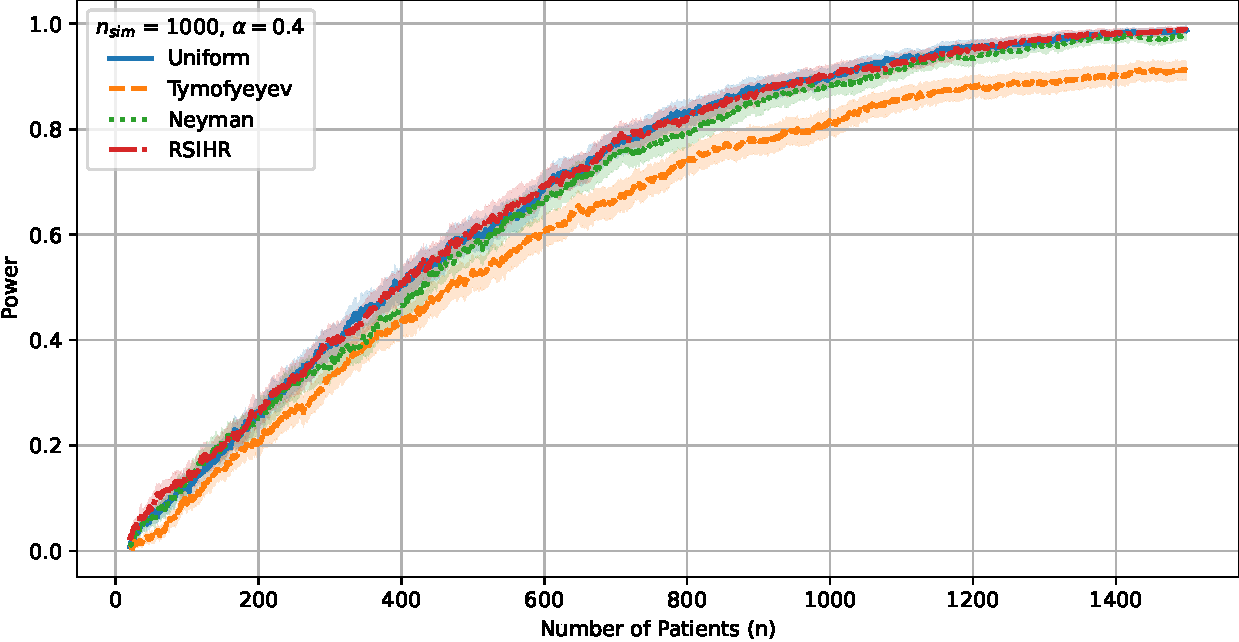
\includegraphics[width=0.7\linewidth]{plots/fixed_targetting/power.pdf}
	\caption{Power profile for fixed Distance Targeting}
	\label{fig:fixed-tgting-power}
\end{figure}


	This last observation is perhaps surprising as we recall that the Tymofyeyev target allocation is the one maximizing the power of this homogeneity test. However, for moderate sample sizes, we observe that a RAR procedure converging to this optimal allocation (even with minimal asymptotic variance) does not necessarily inherit this maximal power.



